% !TeX root=main.tex
\chapter{コマンド体系}

本章では,コントローラボードと FPGA ボードとの間の通信に用いるコマンドについて
説明します.

%%%%%%%%%%%%%%%%%%%%%%%%%%%%%%%%%%%%%%%%%%%%%%%%%%%%%%%%%%%%%%%%%%%%%%%%%%%%%%
\section{コマンドの概要}

SawareruSys におけるコマンドは2つのASCII文字で1セットになっています.コマンドには,
(1) ボードの認識,(2) 出力,(3) 入力 の3種類があります.(1) は,コントローラボード
や FPGA ボードと,対応する Connector アプリとの間で主に使用します.(2) は FPGA
ボードからコントローラボードへと送信され,(3) はコントローラボードから FPGA ボード
に送信されます.Connector アプリは,(2) と (3) のコマンドに対しては中継のみ行います.

表\ref{table:command}に,現在定義されているコマンドを列挙します.コマンドの詳細は
3.2節以降を参照してください.

\begin{table}[hb]
 \centering
  \caption{コマンド定義の一覧表.}
  \label{table:command}
  \begin{tabular}{l|l|l} \hline
      & コマンド     & 定義 \\ \hline \hline
  (1) & V のあとに X & Connector アプリからのボード種別応答要求 \\
      & W のあとに Y & コントローラボードの種別応答 \\
      & v のあとに x & FPGA ボードの種別応答 \\
      & V のあとに Z & すべての入出力状態の再送要求 \\ \hline
  (2) & 0--4         & 出力グループの指定 \\
      & A--H/a--h    & 対応する出力をオン/オフにする \\ \hline
  (3) & I--S, q--r   & 入力の指定 \\
      & U/u          & 対応する入力をオン/オフにする \\ \hline
 \end{tabular}
\end{table}

%%%%%%%%%%%%%%%%%%%%%%%%%%%%%%%%%%%%%%%
\section{ボードの認識に関するコマンド}

ボードの認識に関するコマンドには4種類あります.第1のコマンドは ``VX'' の2文字で,
Connector アプリが接続されたボードに対して,ボードの種類を認識するために送信します.
コントローラボードは,コマンド ``VX'' を受け取ったら,第2のコマンドである ``WY''
で応答します.また,FPGA ボードは,第3のコマンドである ``vx'' で応答します.

Connector アプリはまた,ボードが動作しているかどうかを認識するために,``VX'' を
定期的に送信します.PC 側の Connector アプリはコントローラボードからの応答(``WY'')
を,サーバ側の Connector アプリは FPGA ボードからの応答(``vx'')を,それぞれ一定
時間内に受信できない場合は,タイムアウトとして接続を切断してもよいものとします.

第4のコマンドである ``VZ'' は,Connector アプリが,コントローラボードのすべての入力,
または FPGA ボードのすべての出力の状態を再送してほしいときに送信します.各ボードは,
すべての入力または出力に対してオン・オフのいずれかのコマンドを送信することで,この
コマンドに応答します.

%%%%%%%%%%%%%%%%%%%%%%%%%%%%%%%%%%%%%%%
\section{出力に関するコマンド}

コントローラボードには,8個の LED と4桁の7セグメント LED(小数点を含む)が搭載
されていますので,制御すべき LED の個数は $8 + (7 + 1) \times 4 = 40$ 個になります.
出力に関するコマンドでは,これを8つのセグメントからなるグループ5つで管理します.
コマンド文字列の1文字目では5つのグループいずれかを選択し,2文字目で8つのセグメント
のいずれかをオンまたはオフにします.

\begin{figure}[ht]
 \centering
 \fbox{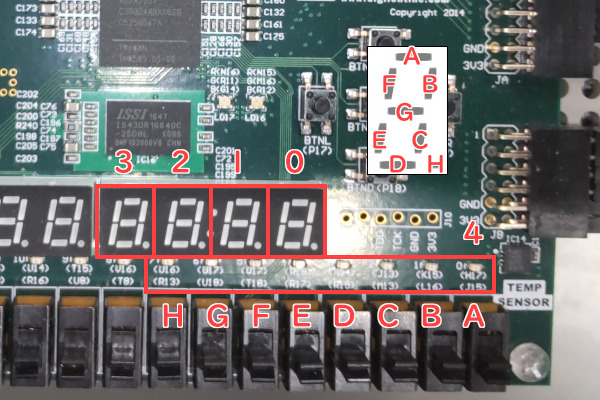
\includegraphics[width=80truemm]{figs/Nexys_LED.jpg}}
 \caption{出力グループおよびセグメントとコマンド文字の対応.}
 \label{fig:Nexys_LED}
\end{figure}

図\ref{fig:Nexys_LED}に,グループおよびセグメントと,対応するコマンド文字との対応を
示します.コントローラボードに図中に記載した文字 A--H のいずれかを送信すると,対応
するセグメントがオンになります.セグメントをオフにする場合には,小文字の a--h を
使用します.例えば,コマンド文字列 ``3G'' は,7セグメント LED の左端の桁の中央の
セグメントを点灯させる,という意味になります.

LED は,PWM 出力やダイナミック点灯により,しばしば頻繁にオン・オフされます.これらに
よって大量の通信が発生することを防ぐため,出力はサンプリングされています.詳細は
4章を参照してください.

%%%%%%%%%%%%%%%%%%%%%%%%%%%%%%%%%%%%%%%
\section{入力に関するコマンド}

コントローラボードには,8個のスライドスイッチと5個(または3個)のタクトスイッチが
搭載されています.入力に関するコマンドではこれらを個別に管理します.
コマンド文字列の1文字目では13個のスイッチいずれかを選択し,2文字目でそのスイッチを
オンまたはオフにします.

\begin{figure}[ht]
 \centering
 \fbox{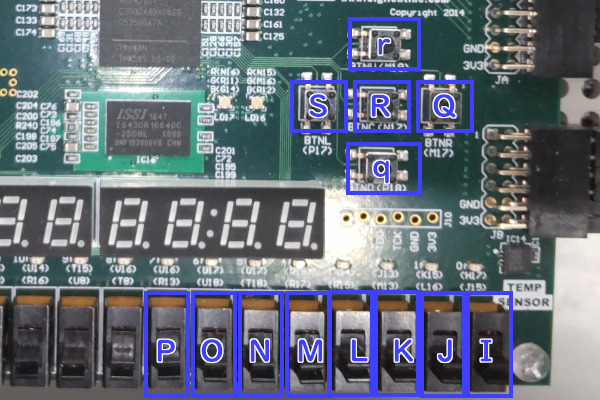
\includegraphics[width=80truemm]{figs/Nexys_SW.jpg}}
 \caption{入力とコマンド文字の対応.}
 \label{fig:Nexys_SW}
\end{figure}

図\ref{fig:Nexys_SW}に,スイッチと対応するコマンド文字との対応を示します.
FPGA ボードに図中に記載した文字 I--S または q,r のいずれかを送信したあと,U を送信
すると,対応するスイッチが仮想的にオンになります.スイッチをオフにする場合には,
小文字の u を使用します.例えば,コマンド文字列 ``SU'' は,左端のスライドスイッチを
オンにする,という意味になります.

%%%%%%%%%%%%%%%%%%%%%%%%%%%%%%%%%%%%%%%%%%%%%%%%%%%%%%%%%%%%%%%%%%%%%%%%%%%%%%